\documentclass[a4paper,12pt]{report}
\usepackage[hidelinks]{hyperref}
\usepackage{graphicx}
\usepackage{float}
\usepackage{caption}
\renewcommand\thesection{\arabic{section}}
\usepackage{array}
\usepackage{tabu}
\usepackage[tt]{titlepic}
%%------------------------------ Title Page -----------------------------------------------
\titlepic{ \centering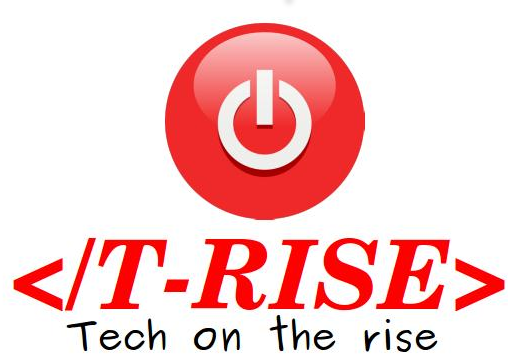
\includegraphics[width=0.7\textwidth]{../images/dddd.png} }
%\documentclass[12pt]{article}
\title{ \rule{\textwidth}{1pt}  \\ \Huge User Manual \\ 
	\Large Cafeteria Management System: Resolve Solution Partners (Pty) Limited \\
	\small Client: Gareth Botha and Jaco Pieterse}
  \author{
         \underline{T-RISE}\\
          Rendani Dau (13381467) \\
	Elana Kuun (12029522) \\
	Semaka Malapane (13081129) \\
	Antonia Michael (13014171) \\
	Isabel Nel (13070305) \\ \\
	https://github.com/toniamichael94/MainProjectCOS301}

\date{\today \\ \rule{\textwidth}{1pt}}

\begin{document}
\maketitle
\break

%% -------------------------------Make table of contents----------------------
\tableofcontents
\break

 \begin{tabu} to 0.8\textwidth { | X[l] | X[l] | }
 \hline
 \textbf{Document Title} & Architectural Specification Document \\
 \hline
 \textbf{Document Identification}  & Document 0.0.3 \\
 \hline
 \textbf{Author}  & Rendani Dau, Isabel Nel, Elana Kuun, Semaka Malapane, Antonia Michael \\
 \hline
 \textbf{Version} & 0.0.3\\
 \hline
 \textbf{Document Status} & Third Version - contains updated architectural requirements \\
 \hline
 \end{tabu}

\begin{table}[h!]
\centering
 \begin{tabular}{||c c c c||} 
 \hline
 \textbf{Version} & \textbf{Date} & \textbf{Summary} & \textbf{Authors} \\ [0.5ex] 
 \hline\hline
 0.0.1 & 29 May 2015 & First draft & Rendani Dau, \\ & & contains & Isabel Nel, \\ & & architectural & Elana Kuun, \\ & & requirements & Semaka Malapane, \\ & & & Antonia Michael \\   [1ex] 
 \hline\hline
 0.0.2 & 30 July 2015 & Second draft & Rendani Dau, \\ & & contains edited & Isabel Nel, \\ & & architectural & Elana Kuun, \\ & & requirements & Semaka Malapane, \\ & & & Antonia Michael \\   [1ex] 
 \hline\hline
 0.0.2 & 25 August 2015 & Third draft & Rendani Dau, \\ & & contains edited & Isabel Nel, \\ & & architectural & Elana Kuun, \\ & & requirements & Semaka Malapane, \\ & & & Antonia Michael \\   [1ex] 
 \hline
 \end{tabular}
\end{table}

\pagebreak

%%now begin document

%%---------------------------------  INTRODUCTION -------------------------------------------
\section{Introduction}
This document contains the architectural requirements for the Resolve Cafeteria Management System that will be created for Software Engineering (COS 301) at the University of Pretoria 2015, by the group T-RISE. In this document we will thoroughly discuss and layout the project's architectural requirements to provide a clear view of the system as a whole.  

%% ------------------------------ VISION ------------------------------------------------------
\section{Vision}
The vision of this project is to implement a fully functional software application that will be maintainable, with detailed supporting documentation and an instruction manual for the Cafeteria Management System. This system will, amongst others, assist in executing orders from the cafeteria, managing the cafeteria's inventory, generating bills, and perform various reporting tasks. 

%%---------------------------------- BACKGROUND -----------------------------------------
\section{Background}
As specified in the project proposal document from Resolve, the cafeteria is currently cash only and does not accept bank cards or electronic payments. This makes it inconvenient for employees as they have to carry around cash if they want to purchase anything from the cafeteria. Employees may choose to go to an external food outlet where they can pay with their preferred method of payment, which uses time and fuel. Lastly, this means the cafeteria does not achieve the maximum amount of income which hinders its growth and improvement.\\

Resolve is therefore looking for a means to accept payments from employees  using their employee access cards or access card numbers, with an amount being deducted from their salary at the end of the month.\\

Resolve proposed the Cafeteria Management System to assist with this problem.
After our first meeting with the client, they brought to our attention that at times the cafeteria does not have enough stock to provide some of the menu items, thus managing the inventory will also be part of the system. The system will predict which inventory items needs to be bought for the next week in order to avoid such a problem. At the end of each month, the bill for the month will be sent to either payroll or to the employee, or both. This option is configurable from the user's profile. The employee can also set a spending limit for each month. There will also be a system wide limit that users cannot exceed.

\section{Architecture Requirements}
The software architecture requirements include the access and integration requirements, quality
requirements, and architectural constraints. These points will be thoroughly discussed below.

%%---------------------------------- ARCHITECTURAL RESPONSIBILITIES----------------------------
\section{Architectural Responsibilities}
\begin{itemize}

\item The system must allow a user to view the menu and select items from the menu without being logged in.
\item The system must allow a user to select items from the menu and place an order when logged in.
\item The system should not process an order unless a user is logged in.
\item On placement of an order the system should send the order details to the cashier.
\item The cashier should be the only party able to notify the user when their order is ready.
\item The cashier should mark the order as paid and collected or just collected when the user collects their order.
\item The system should either send the monthly bill to payroll, the user's personal e-mail address, depending on the preference of the user.
\item The system should allow a user to manage their profile by editing their personal details, password, financial preferences, and spending limit
\item The system should allow configuration and branding by a superuser or an admin user.
\item The system should have the functionality to manage the inventory and the cafeteria (such as the items on the menu and the menu categories). 
\item The system should restrict users to only set their personal maximum monthly spending limits within a range set by the superuser.
\item The system should display the balance of the user on their profile page. 
\item The system should restrict, with the user's consent, that only the financial manager is allowed to view the monthly bill of the user.
\item The system should provide for multiple deployment.
\item The system must be usable, scalable, reliable, and auditable.
\item The system must be maintainable.

\end{itemize}

%% ---------------------------------  QUALITY REQUIREMENTS -------------------------------------
\section{Quality Requirements: Core}

%%--------------SECURITY------------------
\subsection{Security}

\subsubsection{Reasons for security as a quality requirement}
 \begin{itemize}
 \item Security is one of the most important requirements for the Cafeteria Management System. Using the system involves storing confidential details such as personal e-mail addresses, employee IDs, and financial information. The amount the user spends will be deducted from his/her salary, therefore the user must have full control over the amount they can spend. This will be implemented by letting the user set a maximum limit for each month.  
\item There are also super user and admin user roles. Users with these roles have certain functionality assigned to them. These users have access to confidential details of the users and the cafeteria. Other users must not be able to access any functionality besides the functionality assigned to their respective roles. Hence, security is of utmost importance.
 \end{itemize}

 \subsubsection{Strategies to achieve this quality requirement}
 \begin{itemize}
 \item Detecting attacks by determining message integrity, event logging and analysis, scanning for attack signatures and auditing sensitive events (Solms, 2014).
\item Resisting attacks by limiting access and exposure. This can be done by minimizing access channels, minimizing access domains, authentication, confidentiality, assuming external resources as untrusted, minimizing hosting of external resources, additional security layers for valuables. (Solms, 2014).
\item Recovering from attacks by dropping connections and requests. In addition, updating access rules and restoring states.(Solms, 2014).
 \end{itemize}

\subsubsection{Pattern to achieve these strategies}
\begin{itemize}
 \item Layering
\end{itemize}

Layering can enforce security due to separation into layers, in which different users have different levels of access to the layers, depending on their roles in the system

Layering can be used within the subsections of MVC, i.e. the Control and Model layer can be layered to further divide concerns and restrict different users' access on those layers, providing tighter security.

%%-------------USABILITY------------------
\subsection{Usability}

 \subsubsection{Reasons for usability as a quality requirement}
 \begin{itemize}
 \item Usability involves measuring users' performance with regard to the use of a software system. The users of the cafeteria management system will have different technological skill levels, therefore the system has to be user friendly in all aspects and it should not be hard for new users to become familiarized with the system.

 \end{itemize}
 \subsubsection{Strategies to achieve this quality requirement}
 \begin{itemize}
 \item Various goals of usability requirements are firstly, that the interface is intuitive, i.e. easy to navigate and understand, that the buttons and icons are self explanatory for the primary users.
 \item The interface must also not be a cluttered, frustrating and overwhelming one. 
 \item Ease of learning is also an important goal. Users who are unfamiliar with the system, but who have used similar systems in the past, should find the system easy to work with.
 \item The system must also be task efficient, i.e. if users access this space regularly, long tedious processes and other admin must be avoided.
\item Also, the colour schemes, functionality and interactiveness of the interface and system must contribute to this task efficiency. 
\item Different usability tests can be conducted such as handing out paper prototypes of different interface designs, and questionnaires getting feedback from the sample of people that were consulted in the survey. Problems with the different interfaces can be picked up during the usability testing phase, as indicated by the sample of users consulted, such that the final product will be much more user friendly. \url{(http://www.usability.gov/what-and-why/usability-evaluation.html)}

 \end{itemize}
 \subsubsection{Patterns to achieve these strategies}
 \begin{itemize}
 \item MVC
 \item Layering
\end{itemize}
MVC is a suitable pattern because the user will only need to interact with the front end interface, rather than dealing with the technical aspects of the back-end system. Another reason for this is that the developers allocated to working on the View will have the sole focus of making it usable.
Layering can be used within the subsections of MVC, i.e. the Control and Model layer can be layered to further divide concerns and allow different people to work on those layers.


%%-------------RELIABILITY------------------
\subsection{Reliability}
\subsubsection{Reasons for reliability as a quality requirement}
\begin{itemize}
\item The reason we have placed great importance on reliability is because a large scale of users (Resolve employees) will be using the system concurrently in the one hour lunch break thus the system should be able to notify each user separately when their orders are ready and a bill should be generated for each user every month and it  will store the credit made by a user that he/she owes the canteen and reliability of this system of keeping the information safe and correct is thus very important.
\item The system should ensure that the correct amount is deducted from the user's account and that the user's set limits are adhered to.
\item Whilst it may not be possible to design software that is failure and defect-free, software needs to be tested and debugged 
until a satisfactory level of reliability can be achieved, reliability plays a key role, ensuring that all functions work as the user expects them, when the user requires to use the system, thus things like proper unit testing goes hand in hand with reliability.
\item It must hence have a maximum of 2 or 3 hours down time a week (The ideal will be no down time at all, but unfortunately we live in a non-ideal world so one needs to be realistic).
\item The system should be reliable in terms of ensuring that the different functionality is assigned to users with different roles and no user can access functionality outside their role, thus reliability also have a close correlation with security of the system.  
\item Maintenance of a system is also important for reliability, a system must be maintained and kept up to date at all times to ensure that the system stays reliable and any faults found while the system is live should be fixed and the system should be updated thereafter.
\end{itemize}

\subsubsection{Strategies to achieve this quality requirement}
\begin{itemize}
\item Firstly, the prevention of faults. This is done by testing the system thoroughly, using resource locking as well as removing single points of failure (Solms, 2014). We will do this with thorough unit testing on both the client and server side and later on also with proper integration testing between all modules. 
 \item Secondly, detection of faults, which is achieved through deadlock detection, logging, checkpoint evaluation and error communication to name but a few. Recovering from faults also falls under reliability. This is done by passive redundancy, maintaining backups and checkpoint rollbacks. (Solms, 2014)
 \end{itemize}

 \subsubsection{Patterns to achieve these strategies}
 \begin{itemize}
 \item MVC
 \end{itemize}
 The MVC pattern can  be used for reliability, because the different layers are clearly separated, particular teams are focused on working on each layer, making the system more reliable. 

%%-------------AUDITABILITY------------------
 \subsection{Auditability}

 \subsubsection{Reasons for auditability as a quality requirement}
 \begin{itemize}
 \item Any action performed on the system should be traceable back to the person who made these changes and when these changes were made.
 \item In the event of a system crash, it should be possible to roll the system back to a previous working state.
 \item The superuser should be able to view every other user's activities. This is a part of the monitorability aspect of the system.
 \end{itemize}

 \subsubsection{Strategies to achieve this quality requirement}
 \begin{itemize}
 \item System should have log files running at all times to track all transactions made by users. 
 \item Timestamps should be added to document time and date information of the activities done so that the system can trace through the information when needed, such as the events that precede a system crash or unauthorized access
that alters the system in any way.
\item System backup should allow rollback when needed.
\item ACID test can be carried out. Acid is an acronym that describes the properties of a database or system. The properties are:
	\begin{itemize}
	\item \textbf{Atomicity:} Defined as all or none situation referring to the processes that take place on the 
	   system. If something were to go wrong with a process such as posting on the system,
	   then the entire process has to be repeated or not at all.
	\item \textbf{Consistency:} All processes must be completed. No process can be left in a half-finished state,
	     if a failure is detected in a process then the entire process has to be rolled back.
	\item \textbf{Isolation:} Keeps process/transactions separate from one another until they are finished.
	\item \textbf{Durability:} The system must keep a backup of its current state so as to roll back to it if
	    the system where to experience a system failure, crash or corruption of data due
	    to a security breach. (Solms, 2014)
	\end{itemize}
 \end{itemize}

 \subsubsection{Patterns to achieve these strategies}
 \begin{itemize}
 \item MVC
 \item Layering
\end{itemize} 
 MVC is a suitable pattern because it provides auditability through logging all filter inputs and outputs (off queues). Layering is a suitable pattern because each separate layer can be audited and monitored individually, rather than auditing the system as a whole.
  

%%-------------Maintainability------------------
\subsection{Maintainability}
\subsubsection{Reasons for maintainability as a quality requirement}
\begin{itemize}
\item  Maintainability refers to how easily the software can be modified to adapt to a new environment, fix bugs, and improve performance. 
\item Due to the fact that this system is generic enough to be deployed at any cafeteria, this means that a potentially wide range of programmers will be accessing the code and for this reason it is of utmost importance that the code will be easy to grasp and easy to make changes to / maintain.
\item Developers other than those who created the system should be able to add new features, bug fixes, and make changes without investing a significant amount of time and effort in restructuring code and learning/ understanding the code. High level users of the system should also be able to maintain the system without needing to change the code. 

\item Current examples of this requirement in the CMS system are as follows: Firstly, the cafeteria manager can dynamically add menu categories to the menu page and secondly the superuser is able to change various branding options such as the canteen name, the cover image, and the system limit.
\item In addition, the superuser can also change other settings such as being able to change employee IDs as well as assigning roles to various users. There is also an admin user of the system in case the superuser is fired, resigns or deceased.
\item This in turn is not just improving the maintainability of the system, but also the usability of the system.
 \end{itemize}
\subsubsection{Strategies to achieve this quality requirement}
\begin{itemize}
\item Spreading the load across time - queuing (Solms, 2014),
\item Fault detection - deadlock detection (Solms, 2014).
\item Service component publication - naming service and having an interface/contract repository (Solms, 2014).
\item Security tactics such as minimising accessibility (Solms, 2014).
\end{itemize}

\subsubsection{Patterns to achieve these strategies} 
MVC is used to achieve maintainability due to its clean separation of concerns, and organized structure, making it easier for a different programmer to get a high level understanding of the code.  
 

%%-------------SCALABILITY------------------
%\item Scalability
\subsection{Scalability}
\subsubsection{Reasons for scalability as a quality requirement}
\begin{itemize}
\item Scalability refers to a software's ability to handle increased workloads, thus scalability is an important requirement due to the fact that a large volume of Resolve employees will be using the system possibly on the same time each each day (during lunch hour)  and hence the system needs to support all these users concurrently. 
\item In saying this, the system must allow each user to order multiple items and process orders per user concurrently and efficiently.
\item With this, we can assume that there will be an excess of 500 users meaning that the system has to have the ability to handle at least 500 concurrent users at peak times and in a case where the amount of users increase drastically, small server side changes needs to be made with ease to handle more users if needed.
\end{itemize}

\subsubsection{Strategies to achieve this quality requirement}
\begin{itemize}
\item We will need to firstly ensure that existing resources are managed efficiently, i.e. reducing the load using efficient storage, processing,  and persistence (thus the server hosting the system should be efficient enough to handle the current amount of users and more). In addition, we will need to ensure that the load is spread across resources and time, using methods of load balancing to spread load across resources as well as using scheduling and queueing to spread load across time.
\item Secondly, the resources can be scaled up by increasing storage, increasing processing power and increasing the capacity of communication channels (this can easily be done by increasing processing power, and storage space on the server that is hosting the system).
\item Lastly, resources can be scaled out by means of using external resources, using commoditized resources and distributing tasks across specialized resources.
\end{itemize}

\subsubsection{Patterns to achieve these strategies}
\begin{itemize}
\item Concurrency Master-Slave 
\end{itemize}
We chose this pattern here due to the concurrency of the system, meaning that a large number of users must be able to access the system at a time.
%\end{enumerate}

\subsubsection{Strategies to achieve this quality requirement}
\begin{itemize}
\item Unit tests will be conducted, each section of the software needs to be thoroughly tested using unit tests with mock objects ensuring that it works as expected, this includes unit testing on both the client side and the server side.
\item Integration testing will also be conducted on both the client side and server side to ensure that all modules work together as expected.
\end{itemize}

%\end{enumerate}

%%-------------NICE TO HAVE-----------------
\subsection{Nice-To-Have}
Listed below are the nice to have quality requirements related to the Cafeteria Management System, these requirements are not considered as critical but are considered as desirable. \\

\begin{itemize}
\subsubsection{Performance}
\item  Performance refers to the behaviour of the system, meaning its response time and throughput - the number of operations performed per second. The cafeteria system should behave as expected and should not take long to respond. Some changes are important and should be reflected in a timely manner, for example, when an email is sent to a user who forgot his/her password, when an employee id is changed, when an order is ready the user should be notified soon.

\subsubsection{Flexibility}
\item  Flexibility refers to the ability of a system to respond in a time and cost efficient manner to internal or external changes that affects the quality of its service. The system should be able to increase or sustain the quality of its service when responding to these changes.

\subsubsection{Integrability}  
\item  Integrability refers to the ability of the different components of the system to be compatible and pluggable with each other as well as with the components of separate systems. The modules of the cafeteria management system are developed as separate pluggable modules to enforce Integrability. The different modules are integrated together to achieve different functionality, for example a user views the menu (Manage Cafeteria Module), and then proceeds to select a menu item and place an order (Place Order Module). 
 
\subsubsection{Testability} 
\item  It is important to ensure that a software system is adequately tested at various levels. In other words, testing is based on the 
concept of incremental development - during the construction of the system, each added component needs to be thourougly tested to ensure that the functionality works correctly, before it is integrated with the other system components. 
\end{itemize}


%% --------------------------------- ARCHITECTURE REQUIREMENTS ---------------------------------
\section{Access and Integration Requirements}\

%% ---------------- ACCESS CHANNEL REQUIREMENTS ------------
\subsection{Access Channel Requirements}
In this section we will discuss the requirements for the different channels through which the system can be accessed by firstly, people (users - client side) and systems (server-side).


%%------------------HUMAN ACCESS CHANNELS---------------
\subsubsection{Human Access Channels}
The Cafeteria Management System will be accessed by the different users via the online web page (web interface) or through the mobile application. The web interface will be accessible through all the standard web browsers such as Mozilla Firefox, Google Chrome and Microsoft Internet Explorer. The mobile application will be accessible on multiple platforms including the standard IOS/Android platforms. Different services will be available to different users (According to their roles). There are six types of users: Super User, Cafeteria Manager, Cashier, Normal User, Finance and Admin user. These will be discussed below. \\

\paragraph{Superuser\\}
The super user will be one of 2 administrative users that will have global access to all the functionality of the Cafeteria Management System, in particular the super user will have access to the branding of the Cafeteria Management system (changing the logo and so forth) and Administrative settings such as the ability to assign roles to users  . The super user will hence have access to all the functionality of all the other users listed below.

\paragraph{Admin User\\}
The admin user is the second administrative user which will serve as a backup for the super user. The admin user will have all the functionality that the superuser has. 


\paragraph{ Cafeteria Manager\\}
The cafeteria manager will have the ability to view his/her own profile, edit his/her profile, and place orders. This user will also be able to add and edit menu items, view the orders placed by the users of the system, view the inventory, and add or remove inventory. 

\paragraph{ Cashier\\}
The cashier will be able to view his/her profile, edit his/her profile, view the orders placed, and mark off finished orders that are finished and have been collected. The cashier will also be able to make purchases, check inventory and add or remove inventory. Removal of inventory will be done in situations where stock has expired or depleted.

\paragraph{ Normal User\\}
The normal user will be a Resolve employee registered on the Cafeteria Management System.  A normal user will only be able to view his/her profile, edit his/her profile, place orders, check if their order is ready, and view/print their balance reports and account history.

\paragraph{ Finance \\}
The resolve admin user will be able to view all the registered users, their account history and their outstanding balances. This is for administrative and financial purposes . This role has been requested by the Resolve team (the client for this project).

%%------------------SYSTEM ACCESS CHANNELS -----------------
\subsubsection{System Access Channels}
The different technologies selected will be used to support the access channels effectively. We will be using NodeJs running on an Express server and the server needs to be connected to the Mongo database on which various data will be stored and retrieved. This data will be transferred from the server to the respective node modules and so forth. 
The integration channels will also be accessible by the mobile applications, such as Phone Gap, which is the program we will be using to help us convert our web interface into a mobile application.
\begin{itemize}

\item The system will have to integrate with the Mongo database, retrieving information of the employees - such as contact information to notify the user that an order is ready, get inventory or stock and so forth. 

\item The system will also have to integrate with the server to pass information to and from the database.
\end{itemize}

%%------------------PROTOCOLS -----------------------------
\subsection{Protocols}

%%-------HTTP------------
\subsubsection{HTTP - Hypertext Transfer Protocol}
Integration with this protocol will occur at a high level and typically be handled by libraries or browser-clients etc.
\textbf{To be used for:	}
	\begin{itemize}
	\item{All data transferred between users and the server on which the system is hosted, this will be done via the HTTP GET 		and POST requests where we will request data from the database  to be displayed and post data to the database 
		to be stored .}
	\item{Transfer of miscellaneous data such as HTTP error codes to ensure both servers and clients are aware of the state 			of data transfers and its results - in a case of an error we will configure the system to try and rectify the problem 	 		first then when no correction could be made the user will be notified accordingly }
	\end{itemize}

%%----------TCP----------
\subsubsection{TCP - Transmission Control Protocol}
 For establishing network connections between the user computers and the system server. Streams of data can then be exchanged between the connected hosts. Error detection, faulty transmission of data, resending of data etc. will all be done using TCP (Davids). Integration with this protocol will occur at a high level and will typically be handled by libraries or operating system functions.
 
%%------------SMTP--------
\subsubsection{SMTP - Simple Mail Transfer Protocol}
This protocol will be used to handle e-mail communication, specifically notifications to users when their orders are ready, as well as the sending of bills to both users and payroll. It addresses Security as a quality requirement since it incorporates SMTP-Authentication defined by RFC 2554 (Meyers, 1999) which enhances the security of the protocol.

%% ----------------ARCHITECTURE CONSTRAINTS-------------------------
\subsection{Architecture Constraints}

%%--------------TECHNOLOGIES---------------
\subsubsection{Technologies}
Technologies we will be using in the creation of the Cafeteria Management System includes the following: 

\begin{itemize}
 \item \textbf{HTML}: The Software system will be mainly web-based a large part will be made out of HTML5.

 \item \textbf{JavaScript together with AngularJS  and NodeJS}: this will enable us to add extra functionality to our web page and modularise the system thus also helping us to implement dependency injection. For creating reports we will be using \textbf{JSReport} to generate professional invoices displaying the user's bills.

 \item \textbf{CSS together with BootStrap}: which will allow us to style our page and also make it responsive

 \item \textbf{Mongo DB}: MongoDB which is an object oriented database and we will be using it as our database which goes 	
extremely well with NodeJS. 

 \item \textbf{Express server}: will be set up as our server that will host the system.

\item \textbf{MEAN stack}: The MEAN stack is a JavaScript solution that helps you  build fast, robust, and maintainable 	 production web applications using  MongoDB, Express, AngularJS, and  Node.js.

 \item \textbf{Phone gap}: Phone gap will be used to convert our web page into a usable application which will then look like the online webpage that will run like a web interface in the background but  will seem like a mobile application to the user that will be accessible from multiple platforms.

\item \textbf{GitHub}: A version control software and a repository website that will be used to host the source code of the Cafeteria Management System. Reasons for the use of Git is its ease of use, ability to view the entire history of the repo, branch remotely to fix bugs and simultaneously work on various files.  
 \url{(http://git-scm.com/)}.

\end{itemize} 

\subsubsection{Operating Systems}
The Cafeteria Management System will be able to run on all operating systems with standard web browsers such as Mozilla Firefox or Google Chrome.
\section{Architectural Patterns}
For the design of The Cafeteria Management System, the main pattern being used is the  \textbf{MVC (Model-View-Controller) pattern} and the \textbf{Layering architectural pattern}.  Each module of the system has controllers associated with it on the client side as well as server side controllers which are used to access the models containing the declarations of the collections. 
MVC is considered because:
	\begin{itemize}
	\item It provides modularity (i.e. the system's concerns are separated, thus easier to implement). (Solms, 2014)
	\item It allows for better maintainability (one can maintain the Model, View and Controller separately). (Solms, 2014)			\item Testability (it is easier to test because of separated concerns, so the source of any problems are easy to identify). 	
	(Solms, 2014)
	\item Reuse (it is possible to take any component and reuse it where necessary). (Solms, 2014)
	\end{itemize} 
Layering allows the Cafeteria Management System to have pluggable layers, which will allow the developers to replace layers as needed.This pattern allows for: 
		\begin{itemize}
		\item Improved cohesion. (Solms, 2014)
		\item Reduced complexity of the system. (Solms, 2014)
		\item Improved testability (which will allow for easier debugging). (Solms, 2014)
		\item Improved reuse and maintainability of the source code, because all the layers are individual and separate 		
		from 	one another. (Solms, 2014)
		\end{itemize}
However, it should be mentioned that Layering has a performance overhead associated with it, as well as higher maintenance costs associated with the lower layers, because they impact the higher levels. (Solms, 2014). Given the benefits, however, the authors feel that the reduced performance and maintenance costs are a good compromise for reduced complexity and testability.\\
\\ 
 
\newpage
\section{Bibliography}
		\begin{itemize}
			\item \textit{Basic MVC Architecture}. [Online]. Available: <http://www.tutorialspoint.com/struts\_2/\\basic\_mvc\_architecture.htm> [Accessed 5 March 2015].
			
			\item Beal, V. n.d. \textit{Linux Server}. [Online]. Available: <http://www.webopedia.com/TERM/L/\\linux\_server.html> [Accessed 10 March 2015].

			\item Bien, A. 2009. \textit{9 Reasons Why Java EE 6 Will Save Real Money - Or How To Convince Your Management}. [Online]. Available: <http://www.adam-bien.com/roller/abien/entry/\\8\_reasons\_why\_java\_ee> [Accessed 10 March 2015].

			\item Borges, B. 2013. \textit{Reasons to why I'm reconsidering JSF}. [Online]. Available: <http://blog.brunoborges.com.br/2013/01/reasons-to-why-im-reconsidering-jsf.html> [Accessed 10 March 2015].
			
			\item Davids, N.\textit{The Limitations of the Ethernet CRC and TCP/IP checksums for error detection} [Online]. Available: 
			<http://noahdavids.org/self-published/CRC-and-checksum.html>[Accessed 8 March 2015].

			\item \textit{Git --loval-branding-on-the-cheap}. [Online]. Available: <http://git-scm.com/> [Accessed 10 March 2015].

			\item \textit{JavaServer Faces Technology}. [Online]. Available: <http://www.oracle.com/technetwork/\\java/javaee/javaserverfaces-139869.html> [Accessed 10 March 2015].

			\item Kabanov, J. 2011. \textit{Ed Burns on Why JSF is the Most Popular Framework}. [Online]. Available: <http://zeroturnaround.com/rebellabs/ed-burns-on-why-jsf-is-the-most-popular-framework/> [Accessed 10 March 2015].
			\item Meyers, J. 1999. \textit{SMTP Service Extension for Authentication} [Online]. Available: <http://tools.ietf.org/html/rfc2554> [Accessed 9 March 2015]

			\item \textit{Securing FTP using SSH} [Online]. Available: <http://nurdletech.com/linux-notes/ftp/ssh.html> [Accessed 9 March 2015]

			\item \textit{PostgreSQL: About}. [Online]. Available: <http://www.postgresql.org/about/> [Accessed 10 March 2015].
			
			\item \textit{Software Engineering}. [Online]. Available: <http://sesolution.blogspot.com/p/software-engineering-layered-technology.html>[Accessed 5 March 2015].
								
			\item Solms, F. 2014. \textit{Software Architecture Desgin.} [Online]. University of Pretoria: Pretoria. Available: <http://www.cs.up.ac.za/modules/courses/download.php?\\id=8565> [Accessed 9 March 2015].
			
			\item Solms, F. 2015. \textit{Java Persistence API (JPA).} [Online]. University of Pretoria: Pretoria. Available: <http://www.cs.up.ac.za/modules/courses/download.php?\\id=8640> [Accessed 7 March 2015].
			
			\item \textit{SQL Server 2008 R2 Express Database Size Limit Increased to 10GB}. [Online]. Available: <http://blogs.msdn.com/b/sqlexpress/archive/2010/04/21/database-size-limit-increased-to-10gb-in-sql-server-2008-r2-express.aspx> [Accessed 9 March 2015].
			
			\item \textit{Usability Evaluation Basics}. [Online]. Available: <http://www.usability.gov/what-and-why/usability-evaluation.html> [Accessed 5 March 2015].

			\item Wähner, K. n.d. \textit{Why I will use Java EE (JEE, and not J2EE) instead of Spring in new Enterprise Java Projects in 2012}. [Online]. Available: <www.kai-waehner.de/blog/2011/11/21/why-i-will-use-java-ee-jee-and-not-j2ee-instead-of-spring-in-new-enterprise-java-projects-in-2012/> [Accessed 10 March 2015].		

			\item \textit{Welcome to Apache Maven}. [Online]. Available: <http://maven.apache.org/> [Accessed 10 March 2015].
			
			\item \textit{Manageability, Maintainability, and Supportability} [Online]. Available: <https://msdn.microsoft.com/en-us/library/bb896744.aspx> [Accessed 31 July 2015]
			
			

			

		\end{itemize}
\end{document}
